% Chapter Template

\chapter{Literature Review} % Main chapter title

\label{Chapter2} % Change X to a consecutive number; for referencing this chapter elsewhere, use \ref{ChapterX}

\lhead{Chapter 2. \emph{Literature Review}} % Change X to a consecutive number; this is for the header on each page - perhaps a shortened title

%----------------------------------------------------------------------------------------
%	SECTION 1
%----------------------------------------------------------------------------------------

\section{Introduction}
%\begin{figure}[h]
%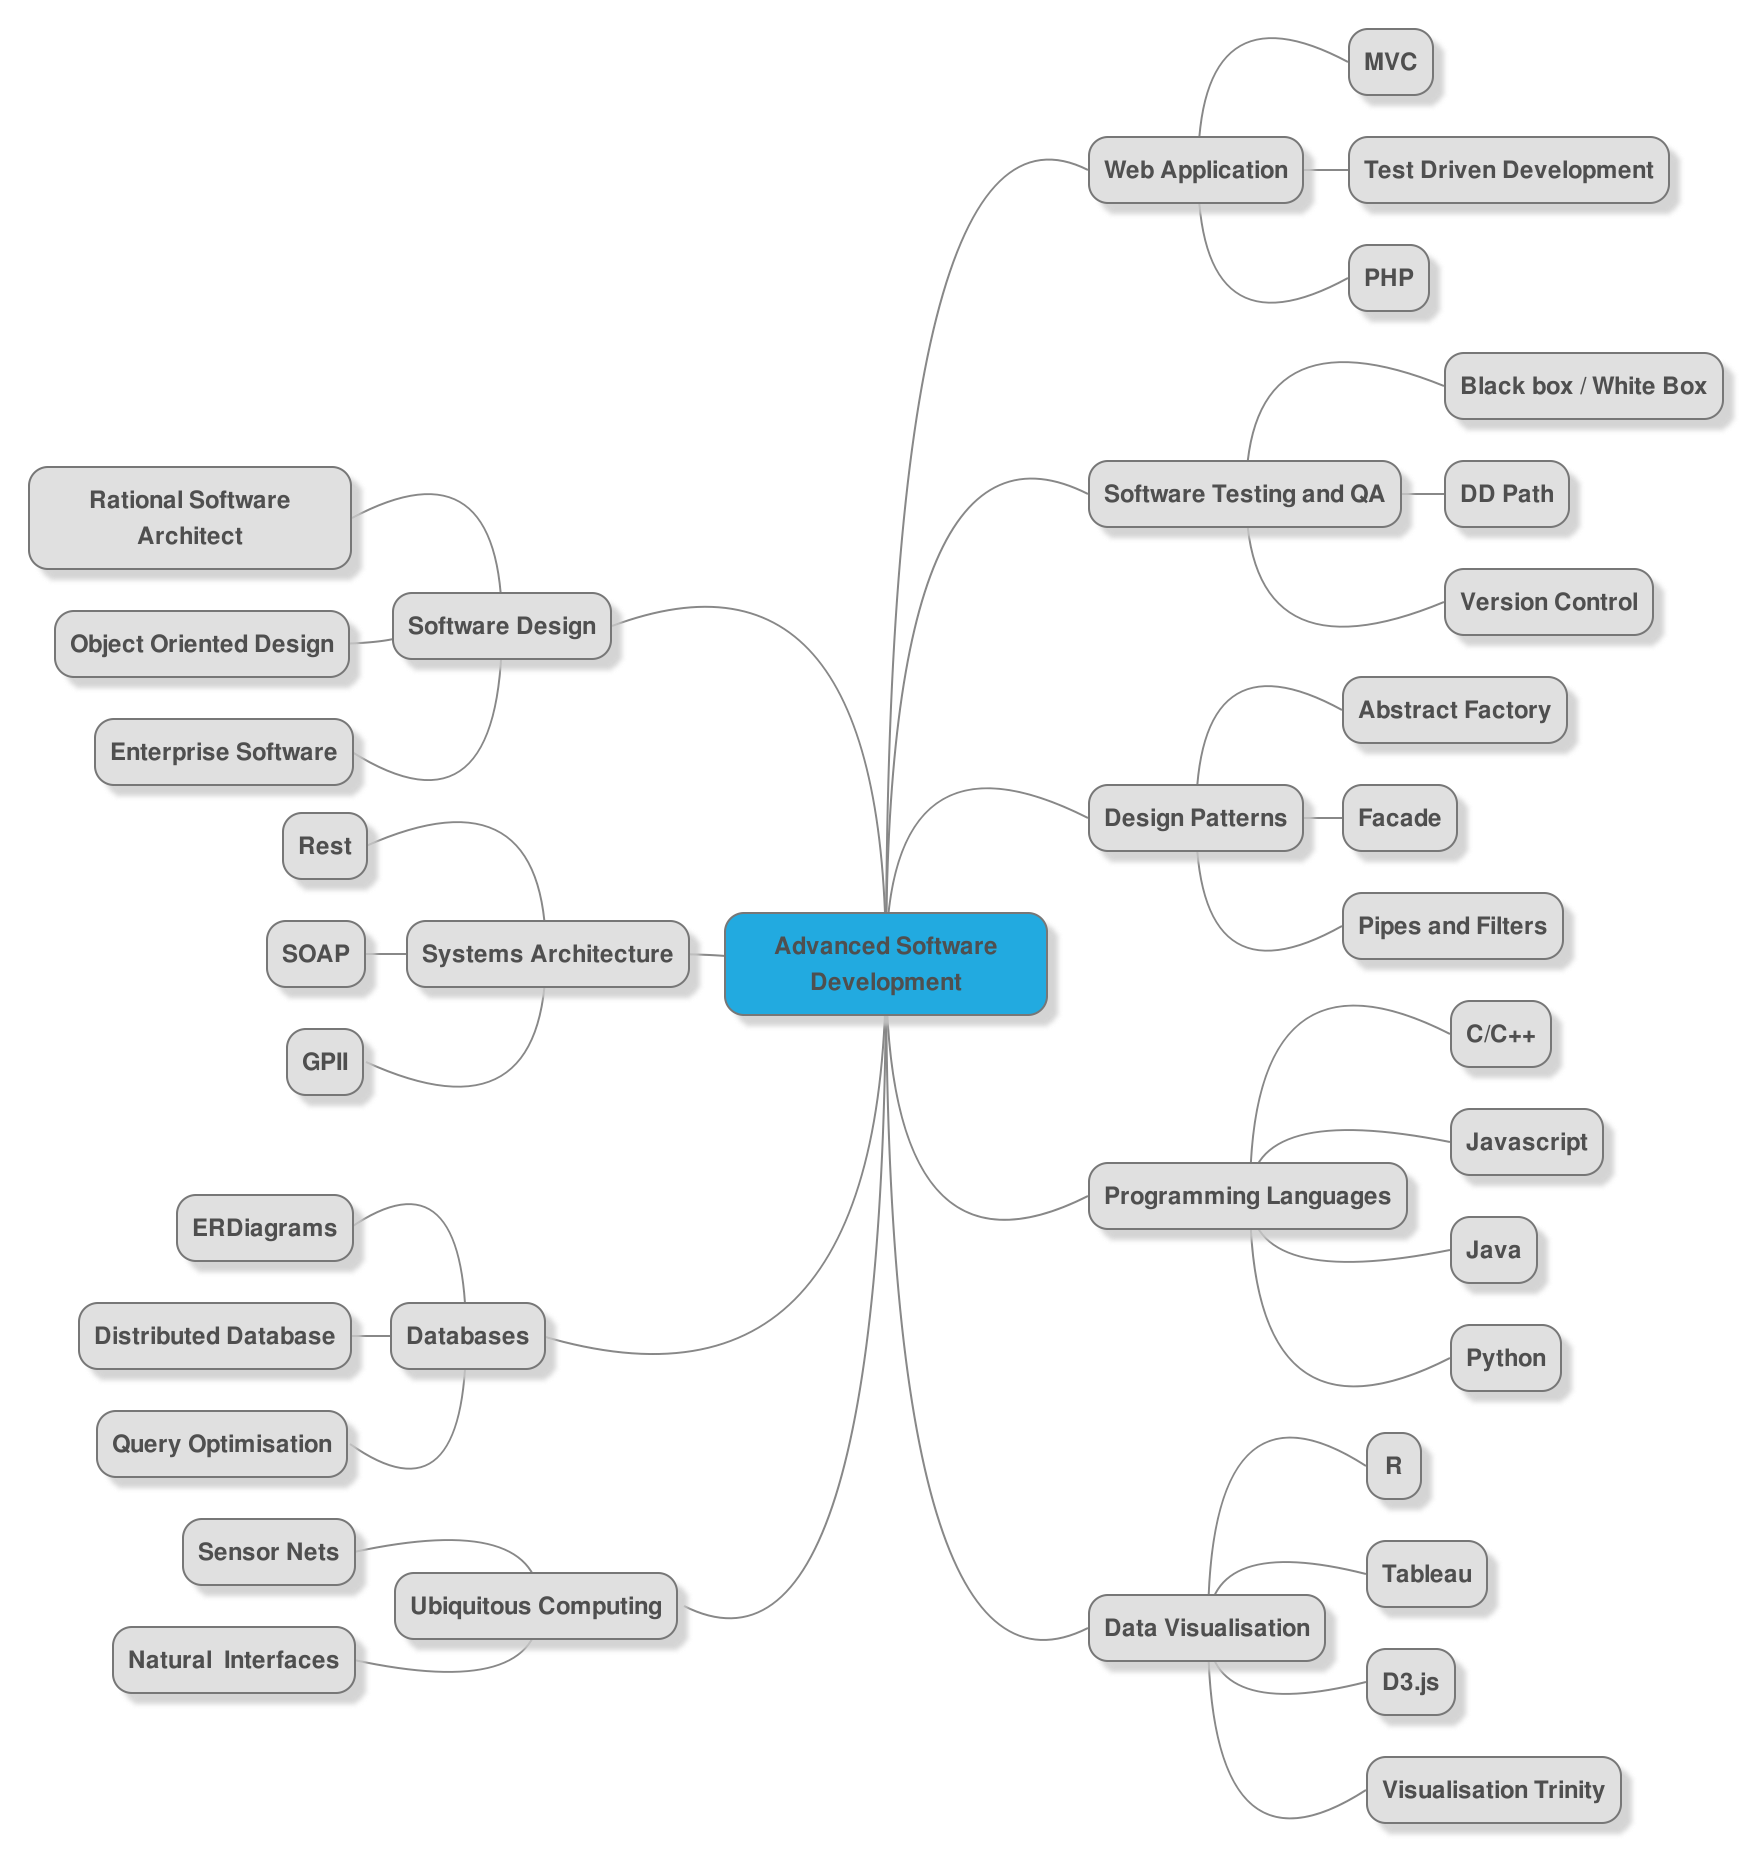
\includegraphics[scale=.2]{mindmap}
%\caption{A mind map of my discipline}
%\centering
%\end{figure}
%-----------------------------------
%	MACHINE LEARNING
%-----------------------------------
\section{Machine Learning}

Supervised learning can be contrasted with unsupervised learning in which the algorithm attempts to find patterns in the data, as opposed to making predictions.

Mitchell (2006) defines machine learning as a field of computer science that attempts to solve the question:

“How can we build computer systems that automatically improve with experience, and what
are the fundamental laws that govern all learning processes?”

Mitchell outlines that while there had been no successful commercial applications of machine learning as late as 1985, it has since been successfully applied in diverse fields such as speech recognition, computer vision, bio-surveillance, robot control and accelerating empirical sciences.

The literature makes the distinction between different learning scenarios. Alpaydin (2004) explains that ‘supervised learning’ happens in a scenario in which the task of the algorithm is to learn the mapping from some input X to an output Y. Examples of supervised learning problems include regression and classification. This could be contrasted with unsupervised learning; described by Mohri, Rostamizadeh and Talwalkar (2012) as problems in which “the learner receives unlabelled training data and makes predictions for all unseen points.” Examples of supervised learning problems include clustering and dimensionality reduction.


\section{Supervised Learning}

Ng (2000) explains that supervised learning algorithms can be divided in regression problems (when the output to be predicted is continuous) and classification problems (when the output to be predicted is discrete). Linear and logistic regression are two machine learning techniques for solving these kinds of supervised learning problems.

\subsection{Regression}

Linear Regression
Non-Linear Regression
Logistic Regression
Regularisation

\subsection{Decision Tables}

Kohavi (1995) proposed decisions tables as a representation for hypothesis in order to solve supervised machine learning problems.

\subsection{Bayesian Networks}

Jensen (1996) explains that Bayesian Networks provide methods for dealing with uncertainty by graphically modelling causal relationships.

\subsection{Artificial Neural Networks}

\subsection{Decision Tree Learning}

\subsection{Support Vector Machines}

\section{Unsupervised Learning}

\subsection{Clustering}

\subsection{K-means}

%-----------------------------------
%	ARGUMENTATION THEORY
%-----------------------------------

\section{Argumentation Theory}

\subsection{Non-Monotonic Reasoning}

\subsection{Defeasible Reasoning}

\subsection{Argumentation Theory in AI}

Dung (1993) was concerned with modelling the fundamental mechanism humans use to argue so as to implement this model on computers. He summarised the basis for his work in the old saying “the one who has the last word laughs best.” In other words, in human typical human argumentation the last piece of evidence to be produced can nullify evidence produced earlier by opposing arguments winning the argument.
He modelled this interaction mathematically as a directed graph; with nodes representing the arguments and edges representing the attack relations between the arguments. This model of arguments and attack relations is known as an argumentation framework.
Within an argumentation framework an argument A can become inadmissible if it is attacked by another argument B. However, if B is attacked by C and becomes in admissible then A may be reinstated.

\subsection{Argumentation Theory Implementations}

%----------------------------------------------------------------------------------------
%	CONCLUSIONS
%----------------------------------------------------------------------------------------

\section{Conclusions}
